\NeedsTeXFormat{LaTeX2e}
\documentclass[12pt, hyperref={pdfpagelabels=false},aspectratio=169,fleqn, greek]{beamer}

\usepackage{amssymb,amsfonts,amsmath,physics}
%resizebox
\usepackage{adjustbox}



% Beamer theme
\usetheme{ntua}

%tikz
\usetikzlibrary{calc,intersections}
\usetikzlibrary{arrows.meta}


\mode<presentation>
\setbeamercovered{transparent=10}
\pgfplotsset{compat=1.16}
% align spacing
\setlength{\jot}{0pt}

%font size of equations
\DeclareMathSizes{12}{9}{10}{10}

%\setbeamertemplate{navigation symbols}{}%remove navigation symbols

\title{Προσομοίωση κίνησης σωματιδίων σε πεδίο ροής ασυμπίεστου, μη συνεκτικού ρευστού}
\subtitle{Πολυφασικές Ροές}
\author{Κωνσταντίνος Μικέδης}
\institute[Εθνικό Μετσόβιο Πολυτεχνείο]{}
\date{24 Φεβρουαρίου 2022}

\begin{document}
\begin{frame}
  \titlepage
\end{frame}


\begin{frame}
  \frametitle{Περιγραφή}
  Πρόβλημα:
  \begin{itemize}
    \item Προσομοίωση κίνησης και εξάτμισης σωματιδίων σε μόνιμο πεδίο ροής
    \item Lagrangian Παρακολούθηση
    \item Μονόδρομη Σύζευξη ($\alpha \ll $)
    \item Εφαρμογή για 2 πεδία ροής 
  \end{itemize}
  Στόχοι:
  \begin{itemize}
    \item Εκτίμηση επίδρασης αριθμού \textit{Stokes} σε κίνηση - εξάτμιση 
    \item Εκτίμηση επίδρασης κίνησης \textit{Brown}
  \end{itemize}
\end{frame}

\begin{frame}
  \frametitle{Περιεχόμενα}
  \begin{enumerate}
    \item Διατύπωση εξισώσεων κατάστασης
    \item Εφαρμογή σε πεδίο ροής με κυψέλες ανακυκλοφορίας (\textit{Maxey})
    \item Εφαρμογή σε ροή γύρω από 2Δ κύλινδρο
    \item Επίδραση δύναμης \textit{Brown}
    \item Εφαρμογή για εξάτμιση
  \end{enumerate}
\end{frame}


\begin{frame}
  \frametitle{\large Εξισώσεις κατάστασης διακριτών σωματιδίων}
  \textbf{Εξίσωση Ορμής:}
  \footnotesize
  \begin{equation}
   \left(m_d + \frac{1}{2} m_c \right) \frac{d v_i}{d t } = 
   \underbrace{(m_d - m_c) g_i}_{\text{βαρύτητα - άνωση}} 
   + 
   \underbrace{m_c u_j \frac{\partial u_i}{\partial x_j} }_{\text{Αδιατάρακτο πεδίο}} 
   +
   \underbrace{3 \pi \mu_c d_p \left(u_i - v_i\right)}_{\text{Αντίσταση Stokes}}
    +
   \underbrace{\frac{1}{2} m_c v_j \frac{\partial u_i}{\partial x_j}}_{\text{Φαινόμενη μάζα}} + \underbrace{F_{B,i}}_{\text{Brown}}\nonumber 
  \end{equation}
  \normalsize
  \textbf{Εξίσωση Συνέχειας:}
  \begin{equation*}
    \frac{dm}{dt} = \mathrm{Sh} \pi d_p D_{AB} (\omega_{A,\infty} - \omega_{A,S})
  \end{equation*}
  \textbf{Εξίσωση Ενέργειας:}
  \begin{equation*}
    mC_p\frac{dT_d}{dt} = \dot{Q}_{conv} + h_{lat} \frac{dm}{dt}
  \end{equation*}
\end{frame}

\begin{frame}
	\frametitle{Πεδίο ροής με ανακυκλφορία}
    \begin{columns}[T]
    	\begin{column}{0.4\textwidth}
			\begin{exampleblock}{Ροϊκή Συνάρτηση}
				\footnotesize
			\renewcommand\arraystretch{1.1}
			$ \psi(x,y) = \alpha U_0 \cos \left(\frac{x}{\alpha}+ \frac{\pi}{2}\right)\sin \left(\frac{y}{\alpha}\right)$
			\end{exampleblock}
			%Ταχύτητα:
			%$\begin{bmatrix}
			%	u_x\\
			%	u_y
			%\end{bmatrix} = 
			%\begin{bmatrix}
			%	\frac{\partial \psi}{\partial y}\\
			%	-\frac{\partial \psi}{\partial x}
			%\end{bmatrix} $
			
			Λόγος ταχυτήτων:
			$$W = \frac{U_t}{U_0} = \frac{(m_p - m_f)g}{3 \pi \mu_c d_p U_0} $$

			Stokes: \quad $St_v = \frac{U_0 \rho_d d_p^2}{\alpha 18 \mu_c}$
			\vspace{0.2cm}\\
			\centering
			$\rho_d/\rho_c >1 \rightarrow \text{Aerosol}$
			$\rho_d/\rho_c <1 \rightarrow \text{Bubble}$
		\end{column}
	
    	\begin{column}{0.6\textwidth}
    		\vspace{-0.7cm}
    		\begin{figure}[ht]
    		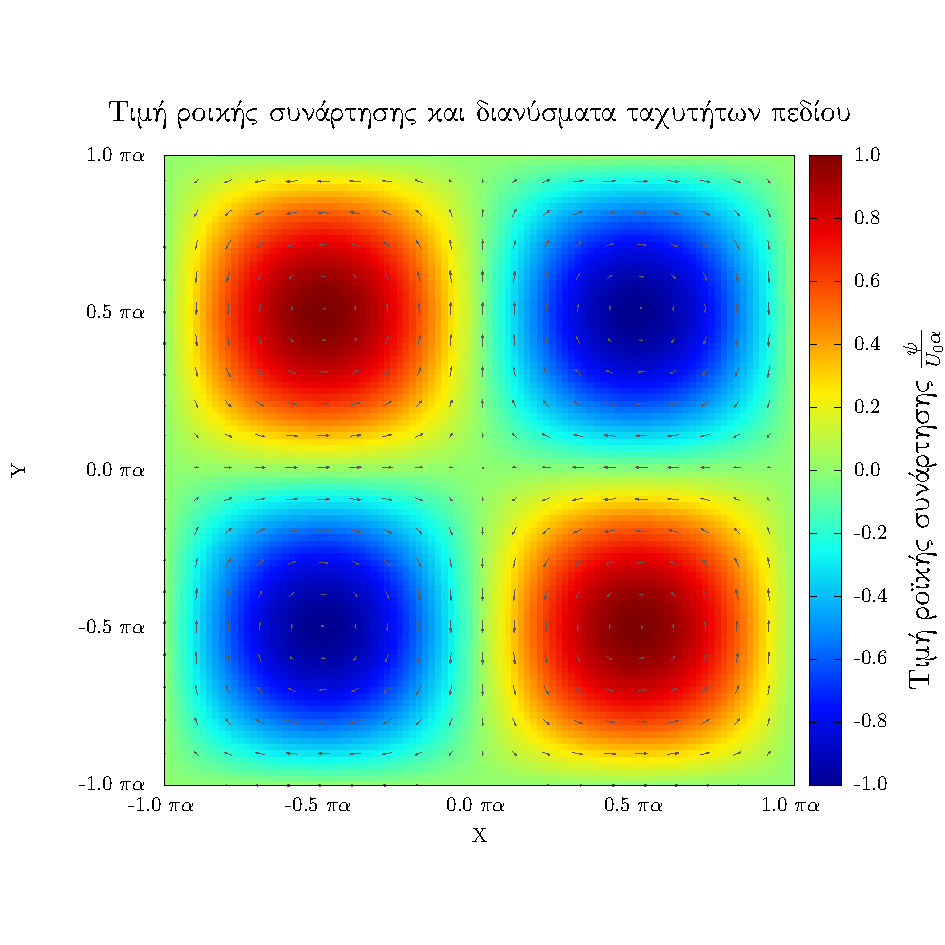
\includegraphics[width = 1.0\textwidth, trim = 1cm 2.0cm 0 1.5cm , clip]{plots/roiki.pdf}
    		\end{figure}
		
   		\end{column}
   	\end{columns}
\end{frame}




\begin{frame}
  \frametitle{Αντιμετώπιση Κρούσης}
	\begin{columns}[c]
		\begin{column}{0.5\textwidth}
			\textbf{Πλήρως ελαστική κρούση}\\
			\bigskip
			Χρόνος κρούσης:
			$$ t_{impact} = \frac{R + d_p/2 - r^n}{v_r} $$ 
			Νέα θέση:
			
			$$\tilde{x_i}^{n+1} = x_i^n + v_i t_{impact} + (v_i + 2n_i n_jv_j ) (\Delta t - t_{impact})$$
		\end{column}

		\begin{column}{0.5\textwidth}
			\vspace{-2.00cm}
			\begin{figure}[h]
				\resizebox{\textwidth}{!}{
					\Large \begin{tikzpicture}
    \coordinate (a) at (-0.405,-1.4);
    \coordinate (b) at (10,0);
    \coordinate (c) at (1,-1);
    \coordinate (o) at (-4,-3);
    
    \draw[name path=circleA] (a) circle (.5cm);
    \draw[thick,black] ([shift=(160:10cm)]10,0) arc (160:200:10cm);
    \draw[dashed,black] ([shift=(160:10.5cm)]10,0) arc (160:200:10.5cm);
    \node [black] at (a) {\textbullet};
    
    
    \draw[-latex] ($(b)+(-4,+0.5)$) --++ (-5.6,2.2) node[midway, below=0.06cm]{$R$};
    
    
    
    \draw[] ($(a) - (-0.25,2) $) --++ (-0.75,6) node[midway, left=0.06cm]{};
    \draw[dotted] ($(a) + (-2,-2)$) --++ (4,4) node[midway, left=0.06cm]{};
    \draw[] ($(a) + (-1.5,-1.5)$) --++ (1.5,1.5) node[midway, left=0.06cm]{$v_i$};
    \node [] at ($(a) + (-2.0,-1.5)$) {$x_i^{n}$};
	\draw[-latex] (a) --++ (-1.2,-0.15) node[near end, above=-0.1cm]{$n_i$};   
    \draw[-latex,dashed] ($(a) $) --++ (1.2,1.2) node[near end, right=0.3cm]{$x_i^{n+1}$};
    \draw[dotted] ($(a) + (+2,-1.3)$) --++ (-4,+2.6) node[midway, left=0.1cm]{};
    \draw[-latex] ($(a)  $) --++ (-1.5,0.975) node[midway, left=0.4cm]{$\tilde{x_i}^{n+1}$};
    
    
    
    
    \draw[black] ([shift=(98:1cm)]-0.405,-1.4) arc (98:147:1cm) node[midway, above=0.1cm] {$\delta$};
    \draw[black] ([shift=(226:1cm)]-0.405,-1.4) arc (226:277:1cm)  node[midway, below=0.1cm] {$\delta$};;
    \end{tikzpicture}}
			\end{figure}

			\end{column}
	\end{columns}
\end{frame}


\begin{frame}
	\frametitle{Εξάτμιση-Συμπύκνωση}	
	\begin{columns}[c]
    	\begin{column}{0.5\textwidth}
			\begin{itemize}
				\item Διακριτοποίηση σε πλέγμα 200$\times$200
				\item Μεταβλητή θερμοκρασία $T_c$
				\item $Ζ=0.005$
				\item Είσοδος σωματιδίων με ρυθμό $\dot{n}$, βάσει $Ζ$
				\item Υπολογισμός μέσων μεγεθών πεδίου και σωματιδίων
				\item Σχετική υγρασία στο περιβάλλον $h_r = 0.0\%$
				\item Πίεση $P_0 = 1~bar$
			\end{itemize}
		\end{column}
    	\begin{column}{0.5\textwidth}
			\vspace{-12pt}
			\begin{exampleblock}{\small Λόγος παροχής μαζών}
				$$ Z = \frac{\dot{m}_d}{\dot{m}_c} = \frac{\dot{n} \frac{1}{6} \pi d_p^3 \rho_d}{A U_0 \rho_c}$$
			\end{exampleblock}
			\begin{exampleblock}{\small Ρυθμός παραγωγής ατμών ανά επιφάνεια}
				\vspace{-12pt}
				$$\left.{\frac{\overline{\frac{dm}{dt}}}{s}}\right|_i = \frac{\sum dm_i}{T s}  = 
				\frac{\sum \frac{dm}{dt}\vert_i \frac{\dot{n} \Delta t}{n_s} }{ s}$$
			\end{exampleblock}
			\begin{exampleblock}{\small Μέση διάμετρος και θερμοκρασία}
				\vspace{-2pt}
				\footnotesize
				$$\overline{T}_i = \frac{\sum\limits_{j=1}^{n_i} T_j}{n_i} \qquad
				\overline{d_p}_i = \frac{\sum\limits_{j=1}^{n_i} d_{p,j}}{n_i}$$
			\end{exampleblock}
   		\end{column}
   	\end{columns}	
\end{frame}

\begin{frame}
	\frametitle{Συμπεράσματα}
	\begin{itemize}
		\item Συμφωνία αποτελεσμάτων με εργασία \textit{Maxey}
		\item \textit{Stokes} $\propto$ Αδράνεια σωματιδίων
		\item O ρυθμός παραγωγής ατμών μειώνεται με αύξηση διαμέτρου 
		\item Πτώση θερμοκρασίας κατά την εξάτμιση
		\item Εσφαλμένη παραδοχή μή αλληλεπίδρασης σωματιδίων
	\end{itemize}
\end{frame}
\end{document}